\documentclass{article}

\usepackage{graphicx}
\usepackage{tabularx}
\usepackage{lastpage}
\usepackage{tikz}
\usetikzlibrary{automata}
\usepackage{qtree}

\date{}
\author{Robert Krency}
\title{Homework 4}

% Geometry 
\usepackage{geometry}
\geometry{letterpaper, left=20mm, top=20mm, right=20mm, bottom=20mm}

% Fancy Header
\usepackage{fancyhdr}
\fancyhf{}
\lhead{CSC 475}
\rhead{Krency}
\cfoot{Page \thepage \hspace{1pt} of \pageref{LastPage}}

% Add vertical spacing to tables
\renewcommand{\arraystretch}{1.4}

% Document
\begin{document}

\maketitle
\thispagestyle{fancy}

\subsection*{Q1 $ L = \{ a^n : n \geq 0  \} \cup \{ b^ma : m \geq 1 \} $}

\begin{figure}[h]
    \begin{center}
    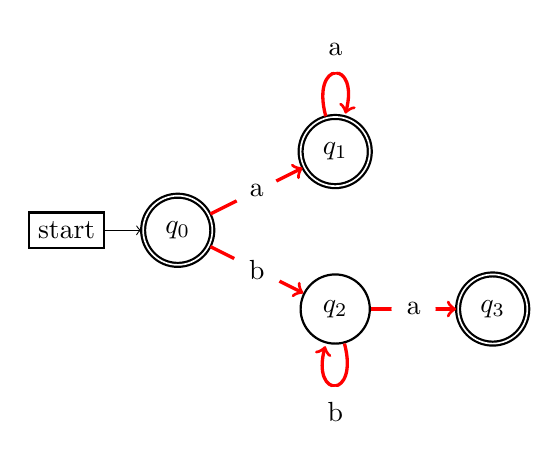
\begin{tikzpicture}
    
        \begin{scope}[every node/.style={circle,thick,draw}]
            \node[initial,state,accepting] (1) at (0,0) {$q_0$};
            \node[state,accepting] (2) at (2,1) {$q_1$};
            \node[state] (3) at (2,-1) {$q_2$};
            \node[state,accepting] (4) at (4,-1) {$q_3$};
        \end{scope}
    
        \begin{scope}[every node/.style={fill=white,circle}, every edge/.style={draw=red,very thick}]
            \path [->] (1) edge node {a} (2);
            \path [->] (2) edge [loop above] node {a} (2);
            \path [->] (1) edge node {b} (3);
            \path [->] (3) edge [loop below] node {b} (3);
            \path [->] (3) edge node {a} (4);
        \end{scope}
    
    \end{tikzpicture}
    
    \end{center}
\end{figure}

\pagebreak

\subsection*{Q2 $L = \{ ab, ba \}^* $}

\begin{figure}[h]
    \begin{center}
    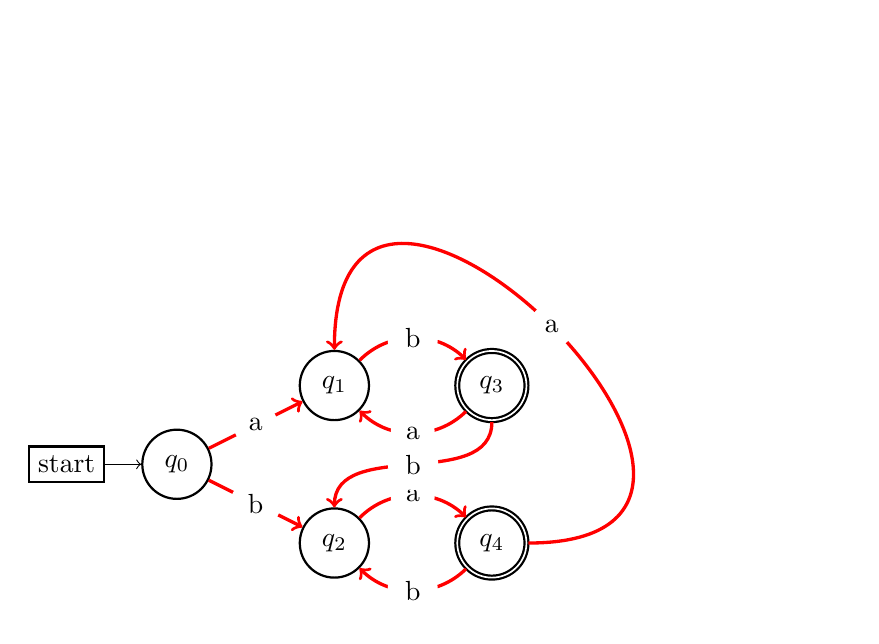
\begin{tikzpicture}
    
        \begin{scope}[every node/.style={circle,thick,draw}]
            \node[initial,state] (1) at (0,0) {$q_0$};
            \node[state] (2) at (2,1) {$q_1$};
            \node[state] (3) at (2,-1) {$q_2$};
            \node[state,accepting] (4) at (4,1) {$q_3$};
            \node[state,accepting] (5) at (4,-1) {$q_4$};
        \end{scope}
    
        \begin{scope}[every node/.style={fill=white,circle}, every edge/.style={draw=red,very thick}]
            \path [->] (1) edge node {a} (2);
            \path [->] (1) edge node {b} (3);

            \path [->] (2) edge [bend left = 45] node {b} (4);

            \path [->] (3) edge [bend left = 45] node {a} (5);

            \path [->] (4) edge [bend left = 45] node {a} (2);
            \path [->] (4) edge [out=270, in=90,looseness=1] node {b} (3);

            \path [->] (5) edge [bend left = 45] node {b} (3);
            \path [->] (5) edge [out=0, in=90, looseness=3] node {a} (2);

            
        \end{scope}
    
    \end{tikzpicture}
    
    \end{center}
\end{figure}


\end{document}